\documentclass[11pt]{article}
\usepackage[top=1.00in, bottom=1.0in, left=1.1in, right=1.1in]{geometry}
\renewcommand{\baselinestretch}{1.1}
\usepackage{graphicx}
\usepackage{natbib}
%\usepackage{gensymb}
\usepackage{amsmath}
\usepackage[utf8]{inputenc}
\usepackage{lineno}
\usepackage{xr-hyper} %refer to Fig.s in another document
\usepackage{hyperref}
\externaldocument{PhenoPhylo_SuppMat}

\def\labelitemi{--}
\renewcommand{\baselinestretch}{1.2}
\parindent=0pt
\parskip=5pt


\title{Phylogenetic estimates of species-level phenology improve ecological forecasting}
% alternative titles:
%% An expanded bayesian phylogenetic mixed model to unravel the phenology-phylogeny tangle. %% this sounds too methodsy
%% Emphasizing species-level differences to unravel the phenology-phylogeny tangle
%% Unravelling the phenology-phylogeny tangle ...
% any other ideas are welcome:


\usepackage{Sweave}
\begin{document}
%\SweaveOpts{concordance=TRUE}


%\bibliographystyle{..//..//refs/bibstyles/naturemag}% 
\author{}
\maketitle

\noindent Authors:\\
Ignacio Morales-Castilla,$^{1}$ T. J. Davies,$^{2,3}$ Geoff Legault,$^{3}$ Daniel M. Buonaiuto,$^{4,5,6}$ Catherine J. Chamberlain,$^{4,5,7}$ Ailene K. Ettinger,$^{8}$ Mira Garner,$^{3,9}$ Faith A. M. Jones,$^{3,10}$ Deirdre Loughnan,$^{3}$ William D. Pearse$^{11}$ \& E. M. Wolkovich$^{3,4,5}$  \vspace{2ex}\\
\emph{Author affiliations:}\\
$^{1}$GloCEE - Global Change Ecology and Evolution Group, Department of Life Sciences, University of Alcal\'a, Alcal\'a de Henares, Spain\\ % (ORCID: 0000-0002-8570-9312)
 $^{2}$Botany, Faculty of Sciences, University of British Columbia, 2424 Main Mall, Vancouver, BC V6T 1Z4, Canada\\
$^{3}$Forest \& Conservation Sciences, Faculty of Forestry, University of British Columbia, 2424 Main Mall, Vancouver, BC V6T 1Z4, Canada\\
$^{4}$Organismic \& Evolutionary Biology, Harvard University, 26 Oxford Street, Cambridge, Massachusetts, USA\\
$^{5}$Arnold Arboretum of Harvard University, 1300 Centre Street, Boston, Massachusetts, USA\\
$^{6}$Department of Environmental Conservation, University of Massachusetts-Amherst, 160 Holdsworth Way, Amherst, MA, USA\\  % 01003
 $^{7}$The Nature Conservancy, 334 Blackwell St Ste 300, Durham, NC, USA \\ %27701
$^{8}$The Nature Conservancy of Washington, 74 Wall Street, Seattle, WA  USA \\ % 98121
$^{9}$Morton Arboretum, USA  \\ 
$^{10}$Department of Wildlife, Fish and Environmental Studies, Swedish University of Agricultural Sciences, 901 83 Umea, Sweden\\ % Faith
$^{11}$ Imperial College, UK\\

\vspace{2ex}
$^*$Corresponding author: ignacio.moralesc@uah.es\\
\renewcommand{\thetable}{\arabic{table}}
\renewcommand{\thefigure}{\arabic{figure}}
\renewcommand{\labelitemi}{$-$}
\setkeys{Gin}{width=0.8\textwidth}

\clearpage



%%%%%%%%%%%%%%%%%%%%%%%%%%%%%%%
% Abstract
%%%%%%%%%%%%%%%%%%%%%%%%%%%%%%%

\section*{Abstract}
Adaptation to ongoing climate change hinges on accurate ecological forecasting to predict shifts in key ecosystem services, such as carbon storage and biodiversity maintenance. Current forecasts, however, have generally failed to capture the important variability in biological responses, especially observed across species.  Here, using novel Bayesian hierarchical phylogenetic models, we overcome this challenge to estimate species-level responses to two major environmental cues of spring phenology: temperature and daylength. We find that variation is greater across species than across cues, suggesting the current focus on identifying which cue is the strongest may be less important than predicting how each species responds to a combination of cues. Further, our model provides insights on how evolutionary history has shaped responses to cues, suggesting stronger evolutionary dynamics in responses to temperature---especially cool winter temperatures---than daylength. Our approach provides a major advance in ecological forecasting, with implications for predicting the impacts of climate change and other anthropogenic forces on species interactions and ecosystem functioning. 
\clearpage



%%%%%%%%%%%%%%%%%%%%%%%%%%%%%%%
% Introduction
%%%%%%%%%%%%%%%%%%%%%%%%%%%%%%%
% Meeting call notes: https://github.com/lizzieinvancouver/ospree/wiki/Phylogeny-and-phenology

% Baby (ecological forecasting), warewolf (species diversity), silver bullet

\linenumbers
\section*{Introduction}
The biological impacts of climate change will have major implications for ecosystem functioning and stability. With rising global temperatures many species have shifted their geographic distributions northward in space and recurring life-history events---their phenology---earlier in time \citep{IPCC:2014sm,parmesan2003}, against a background of high variability. These shifts have cascading consequences on many ecosystem services including carbon storage, making both mitigation and human adaptation to future warming dependent on accurate ecological forecasts. 
% Carbon storage and thus, future climate change itself, depends on accurate forecasts of shifts in plant phenology. But forecasts to date have struggled to reproduce important non-linearities in responses, and the high variability observed in responses to date. 
% Progress towards predicting non-linearities has come from mechanistic models that incorporate multiple predictors. 

While ecological forecasting has improved over recent years \citep{dietze2017ecological,lewis2022power}, it remains a challenge to reproduce the high variability observed in responses to date \citep{IPCC:2014sm}. Some of this variability results from the complexity of climate change itself, including regional and seasonal variation in warming that underlies average trends alongside shifts in other climate axes (e.g. precipitation). Much of it, however, is driven by species-specific variation, reflecting evolved differences in species' sensitivities to underlying environmental cues and their interactions, which we know well for only a few well-studied species \citep{chuinearees,ettinger2020}. In the absence of detailed data on individual species, species groupings (e.g., functional groups) have improved ecosystem models \citep{ed2001,griffith2020}, but still capture only a fraction of the important variability \citep{fuccillo2022}. Improving forecasts, thus, will require models that accurately predict species-level differences in responses to complex environmental change.
% Understanding how different species lineages have evolved their phenotypic responses to the combined effects of environmental change would greatly aid prediction
% IMC - perhaps before <U+00B4>improving forecasts<U+00B4> mention that much forecasting happens at the functional group level (because lack good enough species-level information), hindering insights and biasing forecasts towards those well known species. %EMW29Nov -- got some of this point in, but not all. 

Recent efforts that have attempted to model species-specific responses to the environment \citep{diez2012forecasting} are often confounded by data availability---especially the common problem that data are often prevalent for some species and sparse across others. The rise of Bayesian hierarchical models can allow inference across species in such cases. However, underlying most hierarchical models is an implicit assumption that species are exchangeable \citep{gelman2006}, and they thus partially pool (`shrink') towards estimates for species with the most data and least variable responses, making inference at the species-level unreliable \citep{ettinger2020}. 

Including the evolutionary history of species relationships in models of species responses could at once provide more robust species-level estimates than current approaches and a better understanding of the evolutionary constraints that might limit future adaptation to change. For example, strong phylogenetic niche conservatism \citep{wiens2010niche} could potentially inhibit adaptive responses by drawing species back to an evolutionary conserved optimum, which is sub-optimal under new conditions. More reliable estimates of species-level responses would allow us to better incorporate species differences into models of ecosystem change. 

% JD going nowwhere: Allowing species-level responses to covary over phylogeny might help in identifying ... 

%18Dec2022 -- suggested cut
% Evidence that species' climatic niches show strong evolutionary conservatism \citep{wiens2005niche,olalla2011climatic,morales2020historical}, thus, has major implications for projecting species range shifts, a key response to environmental change \citep{urban353others,gonzalez2016phylogenetic}. More recent work has demonstrated the strength of evolutionary conservatims in species temporal responses, and multiple studies have found dates of budburst, leafout and first flowering are more similar among closely related species \citep{kochmer1986constraints,willis2008phylogenetic,davies2013phylogenetic}. 
%[JD or Nacho add a sentence or two here on how evolutionary responses can be phylogenetically structured for climate change stuff {\bf beyond} phenology and then transition to next paragraph on phenology.]
 
Research using long-term observational data has especially highlighted the role that evolutionary history may play in structuring plant phenological responses---which are critical to accurate forecasts of carbon storage. Phylogenetic signal in plant phenology \citep{kochmer1986constraints,willis2008phylogenetic,davies2013phylogenetic} suggests species responses to cues have diverged over macro-evolutionary timescales, helping explain species present day differences. 
%Almost all these studies, however, have focused on the phenotype (e.g., day of year of a phenological event), which is strongly determined by the local environment (e.g., the climate where phenology was measured). More direct measures of species intrinsic responses to the environment may derive from studies examining species long-term change over time \citep[e.g.,][]{willis2008phylogenetic}---likely capturing a composite of multiple cues---or change per C \citep{yang2021afm}---argued to be a proxy for forcing---and similar metrics, instead of day of year \citep[e.g.,][]{CaraDonna2015}. 
However, approaches using traditional phylogenetic comparative methods, have produced conflicting results \citep[e.g.,][]{willis2008phylogenetic,CaraDonna2015,yang2021afm}. In addition, evidence for phylogenetic conservatism appears to depend on method and species, even varying between sites with overlapping species sets \citep[e.g.,][]{rafferty2017global}, which violates the fundamental idea of shared evolutionary history (the common ancestor of two sets of species cannot possess two separate evolutionary histories for the same trait). A first challenge is thus how to better integrate evolutionary history into multi-species models of plant phenological responses.

Generating robust ecological forecasts requires addressing a second major hurdle---underlying environmental cues that are complex and interacting. Decades of research have informed our understanding of how species use environmental cues to time their phenotypic responses with the temporal distribution of key resources and to avoid periods of high abiotic or biotic stress \citep{larcher1980,bonamour2019}. Commonly, however, responses to environmental cues, and their evolution, are studied individually, linking a given phenotypic response to a single cue, for example, time of leafout responding to summed heat during early spring \citep{davies2013phylogenetic}. These efforts fail to capture the more likely scenario for most phenotypic traits in which multiple cues interacting along evolutionary history have shaped species' responses \citep{Ackerly:2009ly}. For many plant species, phenolological events are determined by a combination of temperature and light \citep{chuinearees}, with additional factors (e.g., other cues or species' physiology) likely further mediating species responses. Although these mediating factors are often less well understood \citep{chuinearees}, they can be accounted for in models either as latent processes or by allowing non-stationarity in responses across species \citep{davies2019phylogenetically}.  

Spring plant phenology may represent our best opportunity to improve forecasts of species' responses to interacting environmental cues. Beyond being the most studied biological impact of climate change, the primary cue system is well established \citep{chuinearees}, especially for temperate woody species where phenology is generally thought to be determined by two components of temperature---chilling (cool temperatures during dormancy period over winter) and forcing (warm temperatures, generally in the spring)---and photoperiod \citep{ospreephoto}. Plant phenology is also one of few phenotypic traits with extensive experimental data on responses to multiple environmental cues across species. Recent multi-species analyses considering forcing, chilling and photoperiod have shown that chilling and forcing together often determine complex non-linear responses to warming, but cannot forecast beyond several well-studied species \citep{ettinger2020}. %These studies have also found remarkable variation across species in their sensitivities to cues, aligning with long-term observational data across thousands of species \citep{XXX}, and suggesting that current models and forecasts fail to capture the complexity of species-specific responses. 

%18Dec2022 -- suggested cut (and lots of re-arranging!) 
% Useful species-level forecasts of phenological responses will require new approaches that better model the evolution of species responses. Our understanding of the underlying cues that drive spring phenology suggest we need to model phenology as a composite outcome of the underlying cues---chilling, forcing and photoperiod---allowing evolution in the responses to each. 
Here we present a novel Bayesian framework that extends upon phylogenetic mixed models \citep{housworth2004phylogenetic} to examine how chilling, forcing (both metrics of temperature) and photoperiod together determine plant phenology. By allowing non-stationarity in species responses across phylogeny \citep{davies2019phylogenetically}, our model departs from most previous work and assumptions of traditional phylogenetic comparative methods \citep[e.g.][]{freckleton2002phylogenetic,ives2011generalized,hadfield2010mcmc}, and moves towards integrating evolutionary history in models of phenological responses to environmental change. To understand how evolution has shaped the cues underlying shifting phenology with climate change \citep{uyeda2017evolution}, we explicitly incorporate phylogenetic structure across model intercepts and slopes (that is, allowing a separate model of evolutionary history for chilling, forcing and photoperiod, see full Methods \& Materials for a complete description). 

We illustrate our method with an unprecedented dataset on phenological responses to environmental cues (chilling, forcing and photoperiod) determined experimentally for 191 deciduous woody species \cite[by far the most studied group of species in phenology experiments, see][]{ettinger2020}, in an updated version of the Observed Spring Phenology Responses in Experimental Environments (OSPREE) database \citep{wolkovich2019}. These data combined with the \citet{smith2018constructing} megatree adjusted to our species and our modeling approach allows us to address the common question of which cue has the largest effect on budburst and at the same time provide robust estimates of how cues vary across species. Using spring phenology, we identify historical regime shifts \citep{uyeda2017evolution} in phenological responses, and highlight how our approach could advance forecasting of other critical responses to ongoing global change.



%%%%%%%%%%%%%%%%%%%%%%%%%%%%%%%
% Results & Discussion
%%%%%%%%%%%%%%%%%%%%%%%%%%%%%%%


\section*{Results \& Discussion}
% Are we in past or present tense here? (asks Lizzie)

Most species respond to all three primary cues---forcing, chilling, and photoperiod \citep[Fig. \ref{fig:muplot_all}, Supporting Table \ref{tab:modelanglamb}, see also][]{Laube:2014a,ettinger2020}---with responses to chilling approximately five-fold greater than to photoperiod (phenological advances of 6.9 days per standardized unit vs 1.2 days, for chilling and photoperiod, respectively; see Table \ref{tab:modelanglamb}). 

These average estimates, however, fail to capture the large differences in species' responses to both chilling and forcing (Fig. \ref{fig:muplot_all}, Supporting Table \ref{tab:tablesupp3}). By allowing species responses to vary based on a model including their shared evolutionary history, we found species differences dwarfed the mean differences between cues, especially temperature cues (Fig. \ref{fig:muplot_all}). The largest in magnitude cue---chilling---varied 25-fold between species, while variation to forcing varied 6-fold. These results suggest the strong current focus on comparing between the three cues may miss the largest variation, and highlights why robust phenological forecasts must account for both the complexity of multiple cues and species-level variation in responses to them. % Or: These results stress the importance of comparing both strength and variation among cues, and highlights why robust phenological forecasts must account for both the complexity of multiple cues and species-level variation in responses to them. 

\emph{Differences across clades \& cues}

The large differences across species produced striking differences between clades. For example, several groups---Oaks and
beeches (Fagaceae), elms (Ulmaceae) and buckthorns (Rhamnaceae)---are highly sensitive to chilling while others---rhododendrons (Ericaceae), butterfly bushes (Scrophulariaceae) or spindles (Celastraceae)---show little to no response to chilling  (Fig. \ref{fig:muplot_all} a). %IMC: not sure if we need some natural history here or some mention to research for some of these clades. Lizzie, if you want to mention-cite something here, please jump in. % EMW (21Nov2022 and 1 Dec2022) I can work with JD to add more here later.
% JD I think some biogeography may be useful here, for example, I think rhododendrons & buddleia are native to the Himalaya, but both are also now widespread and invasive ... need to do a little more digging on the exact species.   
% EMW2023May18 -- I updated to Dan's suggested tecxt
Similar clade-level variation was observed for forcing, where some of these clades---e.g., Ericaceae, Rhamnaceae, Ulmaceae, or Fagaceae---were particularly sensitive (advancing their budburst more than 10 days per standardized unit of forcing) and others such as the Sapindaceae, Cornaceae or Juglandaceae show little response (Fig. \ref{fig:muplot_all} b). %JD - perhaps could link back to invasiveness? Species more sensitive to forcing more invasive? %IMC11Dec - This is a very nice idea... perhaps we can comment on it later in the discussion.
%IMC8May23 - adding here bits from D.Buonaiuto email in case we want to add something more on the biogeography of the clades:
%90\% of extant rhododendron species are evergreen, even though they usually grow in cold mountainous climates. Their diversification rate increased under colder climate conditions and slowed during warmer periods. Increase in monsoon related moisture also is associated with increased diversification. ---- I'm not sure there is much reason why any of these differences should explain different chilling responses except for maybe the evergreen piece, i.e. they don't have a strong chilling cue because they have super cold tolerant leaves inherited from their evergreen uncles and aunts so they're not worried about leafing out too early.





%21Dec2022 -- Lizzie took out the below about frost as I think large chilling cues usually show up in late species (not early-species). 
Some species responded strongly to both temperature cues, which could suggest the existence of syndromes where the genetic basis for responses to one cue---e.g., forcing---has been been selected for alongside responses to another cue---e.g. chilling. This could occur if selection operates on responses to both cues for the same reason; for example, if sensitivity to multiple cues provides greater insurance against leafing out before the last frost \citep{bonamour2019,memegan2021}. Additionally, linkage or pleiotropism among loci associated with different cues \citep{nakagawa2005} could induce these correlations. However, the correlation in species responses across cues was generally weak (\emph{r} = 0.31; between forcing an chilling) and some genera, such as \emph{Tilia} and \emph{Rhododendron} (Ericaceae), displayed strong responses to forcing but weak responses to chilling, while others, such as \emph{Acer} (Sapindaceae), show moderately strong responses to chilling but weak responses to forcing (Fig. \ref{fig:muplot_all}). Species sensitivity to one cue, thus, does not constrain sensitivity to another cue, and it seems selection can operate independently on responses to different cues \citep{bonamour2019}.

In contrast to temperature cues (chilling and forcing) species-level responses to photoperiod were almost uniform across species. This provides novel insight on a large debate over the prevalence of photoperiod cues in temperate trees, where previous experiments \citep{Basler:2012,zohner2016} and models \citep[e.g.,][]{Hunter:1992jw,schaber20203} suggested important variability across species that may constrain the responses of certain species to warming \citep{way2015}. Our results suggest variability is limited to a handful of species in Fagaceae, which have been particularly well studied, especially \emph{Fagus sylvatica} \citep[e.g.,][]{Basler:2012,zohner2016,kramer2017}. As \emph{Fagus sylvatica} is nearly five times more sensitive to photoperiod than most other measured tree species, our results caution against using it to draw inferences of photoperiod responses more widely. These same few species are also where most evidence of local adaptation in photoperiod cues for spring phenology comes from \citep[e.g.,][]{kramer2017}, in contrast with common garden studies of other species, which found little evidence of local adaptation in spring (but not fall) phenology \citep{aitken2016}. The uniformity of response to photoperiod that we found supports this latter view of generally low local adaptation in photoperiod cues for spring phenology (i.e., if local adaptation were high in photoperiod cues we would have expected more variability across species). 

%18Dec2022 -- suggested cut  
% Our results suggest that while chilling and forcing are the dominant cues in terms of the magnitude of their effect sizes (Fig. \ref{fig:muplot_all}), most species are also sensitive to photoperiod, highlighting the potential importance of this cue to both climate change responses in the future, and through evolutionary history. In plants, photoperiod regulates a number of fundamental processes including growth, flowering, stress tolerance, and circadian rhythm \citep{serrano2017,Singh:2017}, with photoperiodic sensing and adaptation to shifting daylength likely occurred early in the evolution of plants, with origins in the green algae \citep{serrano2017}. It is possible, therefore, that phenological responses to photoperiod reflect ancestral sensitivities with origins in deep time. Large plasticity in responses to additional environmental cues (e.g., temperature) for a given photoperiod cue \citep[e.g.,][]{kramer1995} may allow species to track interannual variation in climate with little directional selection on photoperiod sensitivities. Alternatively, photoperiod might thus provide a reliable calibration of the underlying biological clock \citep{jackson2009plant} upon which seasonal variation in climate modifies the tempo. 
%JD - I still need to get to grips with what is going on with photoperiod, low lambda is consistent with rapid evolution within species, but low sigma suggests low rates of evolution. Perhaps photoperiod is dominated by local adaptation, but little directional selection, so local adaptation just gets washed out overtime? 
%IMC11Dec - Would have local adaptation being washed out lead to such a consistent pattern across species? (Lizzie adds -- I think not!)
\emph{Phylogenetic structure of phenological cues}

Variation---or lack thereof---in cues across species and clades provides possible insights into the evolution of cues across the phylogeny. While responses to each cue were phylogenetically structured, with closely related species exhibiting more similar sensitivities than distantly related species, the strength of phylogenetic conservatism in response differs between cues (Fig. \ref{fig:phylosig_all}). Responses to temperature (forcing and chilling) were moderately structured ($\lambda = 0.65$ and $\lambda = 0.54$, for forcing and chilling, respectively). Phylogenetic structure in species responses to photoperiod was comparatively weak ($\lambda= 0.4$) (see Fig. \ref{fig:phylosig_all}, Table \ref{tab:modelanglamb}). % While our approach is unique in focusing on species cues, our results support previous work showing phylogenetic signal in plant phenological timing observed from floras or long-term data \cite{kochmer1986constraints,davies2013phylogenetic}. 

Differences between species in their temperature responses represent shifts in the slope of the relationship between the observed phenology and the cue. The observed phylogenetic structure in temperature responses (forcing and chilling) would be consistent with an interaction with a latent trait that moderates responses, and which also covaries with phylogeny \citep{davies2019phylogenetically}. This fits fundamentally with the idea that early-season phenology plays a critical role in shaping species temporal niches \citep{gotelli1996} and thus should covary with a suite of life-history traits, including whether species are early-active with rapid return on investment traits, or start later in the season and have traits associated with higher competitive abilities \citep[e.g.,][]{Grime:1977sw,memegan2021}. 

%18Dec2022 -- suggested cut  (and re-arrange)
% Geography may drive structured phylogenetic variation, especially in regions where clades have radiated such that close relatives have experienced the same suite of environmental cues and thus been subject to similar selection regimes. Conversely, if species are not generally geographically constrained, as may be more likely the case, especially across deep time \citep{fitzturelli2006}, then we might expect phylogenetic structure in phenology to also weaken, especially when aggregating across locations with different cues \citep{davies2013phylogenetic}.

Weak phylogenetic signal in photoperiod sensitivity (Fig. \ref{fig:phylosig_all}) might seem at odds with the uniformity of species response. However, somewhat counterintuitively, both uniform and random responses can manifest as low phylogenetic signal when indexed by Brownian motion expectations \citep{wiens2010niche}. While rapid local adaptation within species might erase the phylogenetic structure in photoperiod responses, it does not agree with the uniformity we find in species' responses. However, if responses to photoperiod evolved early in plants, as seems likely \citep{serrano2017}, and subsequent selection on photoperiod sensitivity was constrained by stabilizing selection operating on other life-history attributes sensitive to photoperiod \citep[e.g.,][]{Rinne:1994,Wilczek2014,azeez2015}, we would predict both low interspecific variation and weak phylogenetic signal in responses, matching observations. This latter interpretation is also consistent with our estimates of lower $\sigma$ for photoperiod responses (Fig. \ref{fig:phylosig_all}). Here, as in more traditional phylogenetic comparative methods, $\sigma$ represents the rate of evolution, and thus our results suggest photoperiod responses are also evolving slower than temperature responses (see Fig. \ref{fig:burstmodels}).
%18Dec2022 -- suggested cut  
% However, we also show (see Appendix XXX) that an early burst model of evolution, in which trait variation accumulates rapidly early in the history of a clade and then slows through time, consistent with our interpretation of photoperiod evolution.


Phylogenetic conservatism (high $\lambda$) and slow evolutionary rates (low $\sigma$) in traits has sometimes been interpreted as indicative of evolutionary constraints to adaptive change \citep{wiens2010niche,bennett2021evolution}. If this were the case, we might then conclude that species where responses are dominated by forcing cues might be more vulnerable to future warming because phylogenetic conservatism ($\lambda$) in forcing is higher compared to other cues and its evolutionary rate ($\sigma$) is lower than that estimated for chilling. This is misleading, however, as estimates of $\lambda$ are independent from the rate of evolution, and macroevolutionary rates are estimated on phylogenetic trees that integrate across millions of years of evolutionary history, and thus do not necessarily inform us of maximum possible rates of evolution over much shorter timescales. Indeed, there is accumulating evidence for rapid evolution to shifting climates \citep{bradshaw2006,franks2014}. Our estimates are thus more useful in providing unique insights into the evolutionary history of phenological cues, and emphasize the critical importance of incorporating species-level differences in ecological forecasts



\emph{Forecasting species-level responses}

Our results highlight that species-level variability can be extremely high---when properly estimated. Our approach, which partially pooled species responses based on their shared evolutionary history, did not have major effects on the overall average (model slopes for forcing and chilling shifted by 19\% and 21\%, %7.2\% and 3.7\%, I'm using \Sexpr with bzfchange and bzcchange in lines 418-420 from phylo_ospree_compact4_angi... the previous values (7.2, 3.7, come from lines 616-618 in phylo_ospree_plots.R, but they measure departure from the 1-1 PMM-HMM relation so, not quite what we want here. 
respectively; Fig. \ref{fig:correls_angio}), but estimated substantially higher variation across species compared with more widely used hierarchical models. This was especially noticeable in temperature responses (for chilling variance across species means, $\beta_{chill,j}$ in eqn. \ref{modelmu}, was estimated as 23.86 in the phylogenetic model, versus 17.41 in the non-phylogenetic model; variance across means of $\beta_{force,j}$: 8.88 compared to 5.05) while photoperiod, which had low phylogenetic structure, was more similar across approaches (variance across means of $\beta_{photo,j}$: 0.82 compared to 0.62). % The code is now moved to lines 746-752 of phylo_ospree_compact4_angios....R so everything is in the same place; 



The consequences of including shared evolutionary history in forecasting are most apparent for poorly sampled species nested within more well-sampled clades. For example, forecasts for \emph{Acer campestre}, which has only 6 observations, shift by up to 35\% in our phylogenetically informed model compared to one without phylogeny (Fig. \ref{fig:forecast}). In contrast, forecasts for \emph{Betula pendula}, which is one of the most sampled species, are nearly identical across models (Fig. \ref{fig:forecast}). This occurs because cue estimates for \emph{Acer campestre} in the phylogenetically informed model are strongly influenced by other \emph{Acer} species, which diverge from other clades. In the non-phylogenwtically informed model all species are equally exchangeable and thus \emph{Acer campestre} is pulled strongly towards well-sampled species, such as \emph{Betula pendula} ($n = 311$), leading to forecasted shifts that are more similar across all species---especially poorly sampled species (Fig. \ref{fig:forecast}). 

The increase in variability across species in our model with phylogenetic structure also decreased the uncertainty in estimates for each individual species temperature responses (Fig. \ref{fig:suppuncertainties}). Thus, traditional (non-phylogenetically informed) approaches that partially pool across species (most hierarchical models in ecology) may also lead to less precise predictions and forecasts of phenology for individual species, although overall model accuracy might still appear reasonable (see Fig. \ref{fig:accuracycomp})).
%21Dec2022 -- ref new supp figure later (instead of the below that I commented out)
% The increase in variability across species in our model with phylogenetic structure decreased the uncertainty in estimates for each individual species temperature responses (by 6\% for chilling, 6\% for forcing and 2\% for photoperiod)

% Counterintuitively, induced reductions in cross-species variance, far from increasing estimation accuracy could lead to increased type-II error by failing to detect actual relationships among cue and responses that would only emerge when phylogeny is correctly accounted for (see Supporting Information XX). % EMWDec1 -- I am not sure what we mean in this last sentence, but it sounds important ... but since I am not sure what we mean I apologize if I put it in the wrong place... Update %18Dec2022 -- I suggest that we cut it.  

%18Dec2022 -- suggested cut  
% Our results could help inform which clades will be more sensitive to different axes of climate change---e.g., changes temperatures over winter (associated with chilling) versus spring (associated with forcing). For example, using a hierarchical model would not have identified oaks (genus \emph{Quercus}) as being among the most sensitive taxa to forcing and chilling (see e.g., \citep{ettinger2020}), but we show that, on average, species within this genus advance phenology by -13.09 days per standard unit of forcing and -17.33 days per standard unit of chilling. Hierarchical models, even if non-phylogenetic ($\lambda$ = 0), would also capture oak phenological advances as a response to forcing (-11.14 days per standard unit) and chilling (-13.36 days per standard unit). These results highlight the need to move beyond current very general classifications currently used in models \citep[e.g., functional groups ... Cat/Dan, can you offer better ref?][]{Moorcroft:2003dz} or groupings at coarse taxonomic levels \citep[e.g.,][]{ettinger2020} to make improved ecological forecasts for individual species. 

The contrasts between temperature sensitivities and photoperiod sensitivities---in both their variability across species and phylogenetic structure---have important implications for generating multi-species forecasts. Notably, photoperiod cues appear weaker, more uniform across species, and less phylogenetically constrained than temperature cues. For temperature responses, the large variability among species makes predicting species individual responses challenging, but the phylogenetic structure in responses lets us borrow information from close relatives to improve our predictions. However, given that Brownian motion (our assumed model of evolution) is an extremely noisy process, we recommend imputation \citep{molina2018assessing} only for missing taxa that are closely related to other well sampled species or clades.
% While this must be done with care , our results could provide reasonable predictions for many temperate woody plant species from clades for which we have multiple species and experimental observations at varying treatment levels (e.g., Betulaceae),. 

% For photoperiod, the weak phylogenetic structure in responses indicates that phylogeny retains little information, but because species responses are generally more uniform, we can be more confident in assuming the mean species response across species, comforted in the knowledge that small errors will likely not have large impact given the relatively weak overall contribution of this cue, except for \emph{Fagus sylvatica}.
% The genus \emph{Fagus} is recognized as being particularly sensitive to photoperiod \citep{fu2019}. Specifically, \emph{Fagus sylvatica} is nearly five times more sensitive to photoperiod than most other measured tree species. The question arises as to whether species with outlying responses should be chosen as the model from which to extrapolate knowledge as done with \emph{Fagus sylvatica} in the phenology literature (REFs for PEP75?!). %HELP with references on Fagus would be appreciated. % EMW (21Nov2022) I'll add more here later

While we focused on spring phenology here, our approach suggests a path forward for more general forecasting of species-level climate change responses. Our results show how including the phylogenetic relationship of species in a mechanistic model of underlying cues can overcome major limitations of most current hierarchical models---producing biased model estimates, underestimating the full variability across species, and increasing uncertainty around individual species' estimates---while at once providing insight into the evolutionary history of biological responses. Using this approach improved forecasts of biological responses to climate change and could help anticipate impacts on critical ecosystem services from species-level shifts and thus aid mitigation and human adaption to warming. 


%%%%%%%%%%%%%%%%%%%%%%%%%%%%%%%
% Longer Methods and Materials
%%%%%%%%%%%%%%%%%%%%%%%%%%%%%%%


\clearpage
\section*{Methods \& Materials} 
\iffalse
Chunks to maybe work in... 
\begin{itemize}
\item Common phylogenetic regression accounts for phylogenetic relationships as a grouping factor either explicitly (PMM) or implicitly (PGLS). Here we present one possible approach that accounts for more complex interactions going on among predictors, which would be reflected in the species-level slopes being allowed to vary as a function of the phylogeny, rather than keeping slopes constant and only allowing the intercepts (or residuals) to vary. 
\item In a first attempt at establishing whether or not it is important, we compare results from a common hierarchical model with partial pooling on the slopes that does not allow for phylogenetic constraints to affect slope estimates against results from a phylogenetic hierarchical model allowing phylogeny to constrain partially pooled slopes. 
\end{itemize}
\fi
\subsection*{Phenological and Phylogenetic Data}
% See _README_paperresearchmethods.txt
\emph{Phenological data:} To estimate phenological responses to chilling, forcing and photoperiod we used data from phenological experiments in controlled environments of temperate woody species, brought together in the Observed Spring Phenology Responses in Experimental Environments (OSPREE) database. In July 2019, we updated an earlier version of this database \citep{wolkovich2019} by reviewing all papers found through searching ISI Web of Science and Google Scholar with the following terms: 
\begin{enumerate}
\item TOPIC = (budburst OR leaf-out) AND (photoperiod OR daylength) AND temperature*, which yielded 623 publications
\item TOPIC = (budburst OR leaf-out) AND dorman*, which yielded 270 publications
\end{enumerate}
We scraped data from all papers of woody species that tested for photoperiod and/or temperature effects on budburst, leafout, or flowering, resulting in 56 papers. \citet{ettinger2020} used a portion (72 experiments across 49 papers) of the earlier OSPREE database and provides extensive methods on the database creation and cleaning. For our analysis here, we included all budburst experiments where we could quantify chilling, forcing and photoperiod levels, resulting in 44 studies from 33 papers. We focused on angiosperms as gymnosperms are very poorly represented in spring phenology experiments. 
% Nacho, please:
% XX add length(unique(datasetID)) from an OSPREE clean file (make sure it does not have strawberries). 
% YY add length(unique(paste(datasetID, study)) from datafile you use in the end ... ditto for ZZ
% Also, we need to publish an updated OSPREE dataset on KNB eventually.

Across experiments chilling treatments were often fully or partially applied in the field, thus we estimated field chilling ourselves in Utah units with the \verb|chillR| package combined with daily temperature data (converted to hourly) from both European \citep[E-OBS, version 16, calculating the average of minimum and maximum daily temps,][]{cornes2018} and North American \citep[v3,][]{princetonclimate} gridded climate datasets. \citet{ettinger2020} provides additional details on these calculations (however, to have climate data through all study years given the updated OSPREE database, we used a different climate dataset here for North America).
% We could probably add species info above? If you want to contrast with bb ms: \citet{ettinger2020} had 39 years, and 203 species
% Lizzie says ... this methods part feels a little short to me, but I think it may be all we need. (Maybe Ailene can eventually take a look to check what might be missing? But I think we can definitely wait for that until we have a full draft.)
% IMC - I may need help from Cat about the latest chilling data sources, the metric and so on. It will be great to have Ailene double-checking this part.

For a phylogenetic tree, we pruned  the phylogenetic megatree for seed plants \citep{smith2018constructing} to extract a subset of the phylogenetic tree containing only the angiosperm species in the OSPREE dataset, then added species that were not present in the megatree as polytomies at the generic level \citep[using the function `congeneric.merge' in][]{pearse2015pez}), with a branch length of zero. Polytomies represent 26.8\% of the full angiosperm dataset. To test for the ability of polytomies to bias our results we run sensitivity analyses excluding these species from models (which lead to 142 angiosperms; see Supporting Information). \\ 

\subsection*{Bayesian hierarchical phylogenetic model}
% PICs are also sort of a regression phylo thing so adjusted below ..
Commonly used phylogenetic regression methods today (e.g., PGLS and PMM) were originally conceived as statistical corrections for phylogenetic non-independence across observations---generally species---thus allowing multi-species studies to meet the assumptions of linear regression \citep{freckleton2002phylogenetic}. These corrections incorporated phylogenetic structure in the regression by modifying the residual variance-covariance matrix to substitute off-diagonal elements of zero (the value given the assumption of independence across observations) for shared phylogenetic branch lengths representing pairwise covariances (under phylogenetic non-independece among observations). Off-diagonals were also allowed to include a multiplying parameter---generally referred to as $\lambda$---which is a transformation indicating the amount of phylogenetic relatedness among species (see below). Because the original aim of these methods was to correct for statistical nuance, the underlying assumption of phylogenetic regressions is that phylogenetic relatedness would only affect either model residuals \citep[in PGLS approaches,][]{freckleton2002phylogenetic} or the model intercepts \citep[e.g., in many PMM approaches,][]{housworth2004phylogenetic}.
% IMCmar04 - It would be great to have others (Lizzie, Jonathan and/or Will)reviewing this paragraph to double-check it is accurate

Because our aim is to understand how evolution may have imprinted biological responses to multiple interactive cues, our approach expands the above methods by explicitly incorporating phylogenetic structure across model intercepts and slopes. Doing so allows explicitly estimating the amount of phylogenetic relatedness in species' sensitivities to each cue, when these sensitivities are modelled in a multi-predictor regression setting.  
% IMCmar04 - starting to flesh out this bit. Needs work.
% EMW (13Mar2022): May want to add a supplement explaining how intercepts and residuals are somewhat similar in our model? Especially as you touch on it above. Geoff has some text for this. 

% The following text is copied from Geoff's PMM description:
For each observation $i$ of species $j$, we assumed that the timing of phenological events were generated from the following sampling distribution:

\begin{align}
  \label{modely}
  y_{i,j} \sim \mathcal{N}(\mu_j, \sigma_e^2)
\end{align}
where
\begin{align}
  \label{modelmu}
  \mu_j = \alpha_j + \beta_{chill,j} X_{chill} + \beta_{force,j} X_{force} + \beta_{photo,j} X_{photo}
\end{align}
and $\sigma_e^2$ represents random error unrelated to the phylogeny. 

Predictors $X_{chill}$, $X_{force}$, $X_{photo}$ are standardized chilling, forcing, and photoperiod, and their effects on the phenology of species $j$ are determined by parameters $\beta_{chill,j}$, $\beta_{force,j}$, $\beta_{photo,j}$, representing species' responses (or sensitivities) to each of the cues. These responses, including the species-specific intercept $\alpha_j$, are elements of the following normal random vectors:

\begin{align}
    \label{phybetas}
  \boldsymbol{\alpha} = [\alpha_1, \ldots, \alpha_n]^T & \text{ such that }
  \boldsymbol{\alpha} \sim \mathcal{N}(\mu_{\alpha},\boldsymbol{\Sigma_{\alpha}}) \\
  \boldsymbol{\beta_{chill}} =  [\beta_{chill,1}, \ldots, \beta_{chill,n}]^T & \text{ such that }
  \boldsymbol{\beta_{chill}} \sim \mathcal{N}(\mu_{\beta_{chill}},\boldsymbol{\Sigma_{\beta_{chill}}}) \nonumber \\
  \boldsymbol{\beta_{force}} =  [\beta_{force,1}, \ldots, \beta_{force,n}]^T & \text{ such that }
  \boldsymbol{\beta_{force}} \sim \mathcal{N}(\mu_{\beta_{force}},\boldsymbol{\Sigma_{\beta_{force}}}) \nonumber \\
  \boldsymbol{\beta_{photo}} =  [\beta_{photo,1}, \ldots, \beta_{photo,n}]^T & \text{ such that }
  \boldsymbol{\beta_{photo}} \sim \mathcal{N}(\mu_{\beta_{photo}},\boldsymbol{\Sigma_{\beta_{photo}}}) \nonumber
\end{align}

\noindent where the means of the multivariate normal distributions are root trait values (i.e., values of cue responses prior to evolving across a phylogenetic tree) and $\boldsymbol{\Sigma_i}$ % we need to decide for a nomenclature that is as widespread/easy to understand as possible. Other papers use bold V, or C to refer to the VCV matrix. Any suggestions are welcome
are $n \times n$ phylogenetic variance-covariance matrices of the form: \\ 
\begin{align}
  \label{phymat}
\begin{bmatrix}
  \sigma^2_i & \lambda_i \times \sigma_{i} \times \rho_{12} & \ldots & \lambda_i \times \sigma_{i} \times \rho_{1n} \\
  \lambda_i \times \sigma_i \times \rho_{21} & \sigma^2_i & \ldots & \lambda_i \times \sigma_{i} \times \rho_{2n} \\
  \vdots & \vdots & \ddots & \vdots \\
  \lambda_i \times \sigma_i \times \rho_{n1} & \lambda_i \times \sigma_i \times \rho_{n2} & \ldots & \sigma^2_i \\
\end{bmatrix}
\end{align}

\noindent where $\sigma_i^2$ is the rate of evolution across a tree for trait $i$ (here assumed to be constant along all branches), $\lambda_i$ scales branch lengths and therefore is a measure of the ``phylogenetic signal'' or extent of phylogenetic relatedness on each model parameter (i.e., $\alpha_{j}$, $\beta_{force,j}$, $\beta_{force,j}$, $\beta_{photo,j}$), and $\rho_{xy}$ is the phylogenetic correlation between species $x$ and $y$, or the fraction of the tree shared by the two species.

The above specification is equivalent to writing equation \ref{modelmu} in terms of root trait values and residuals, such that:

\begin{align}
  \label{eqfive}
  \mu_j = \mu_\alpha + \mu_{\beta_{chill}} X_{chill} + \mu_{\beta_{force}} X_{force} + \mu_{\beta_{photo}} X_{photo} + e_{\alpha_{j}} + e_{\beta_{force,j}} + e_{\beta_{chill,j}} + e_{\beta_{photo,j}}
\end{align}

\noindent where the residual phylogenetic error terms (e.g., $e_{\alpha_{j}}$) are elements of normal random vectors from multivariate normal distributions centered on $0$ with the same phylogenetic variance-covariance matrices as in equation \ref{phymat}. Model code, including priors used here, are given in the supplement. 





\bibliography{phylorefs}
\bibliographystyle{amnat}


%%%%%%%%%%%%%%%%%%%%%%%%%%%%%%%
% Tables and Figures
%%%%%%%%%%%%%%%%%%%%%%%%%%%%%%%
\clearpage
\section*{Tables and Figures} 


%IMC 22mar - we should decide among one of the next two figures, instead of having separate figures per cues?
% EMW (28Mar2022): I vote for the first one, but both are great!
\begin{figure} 
  \begin{center}
  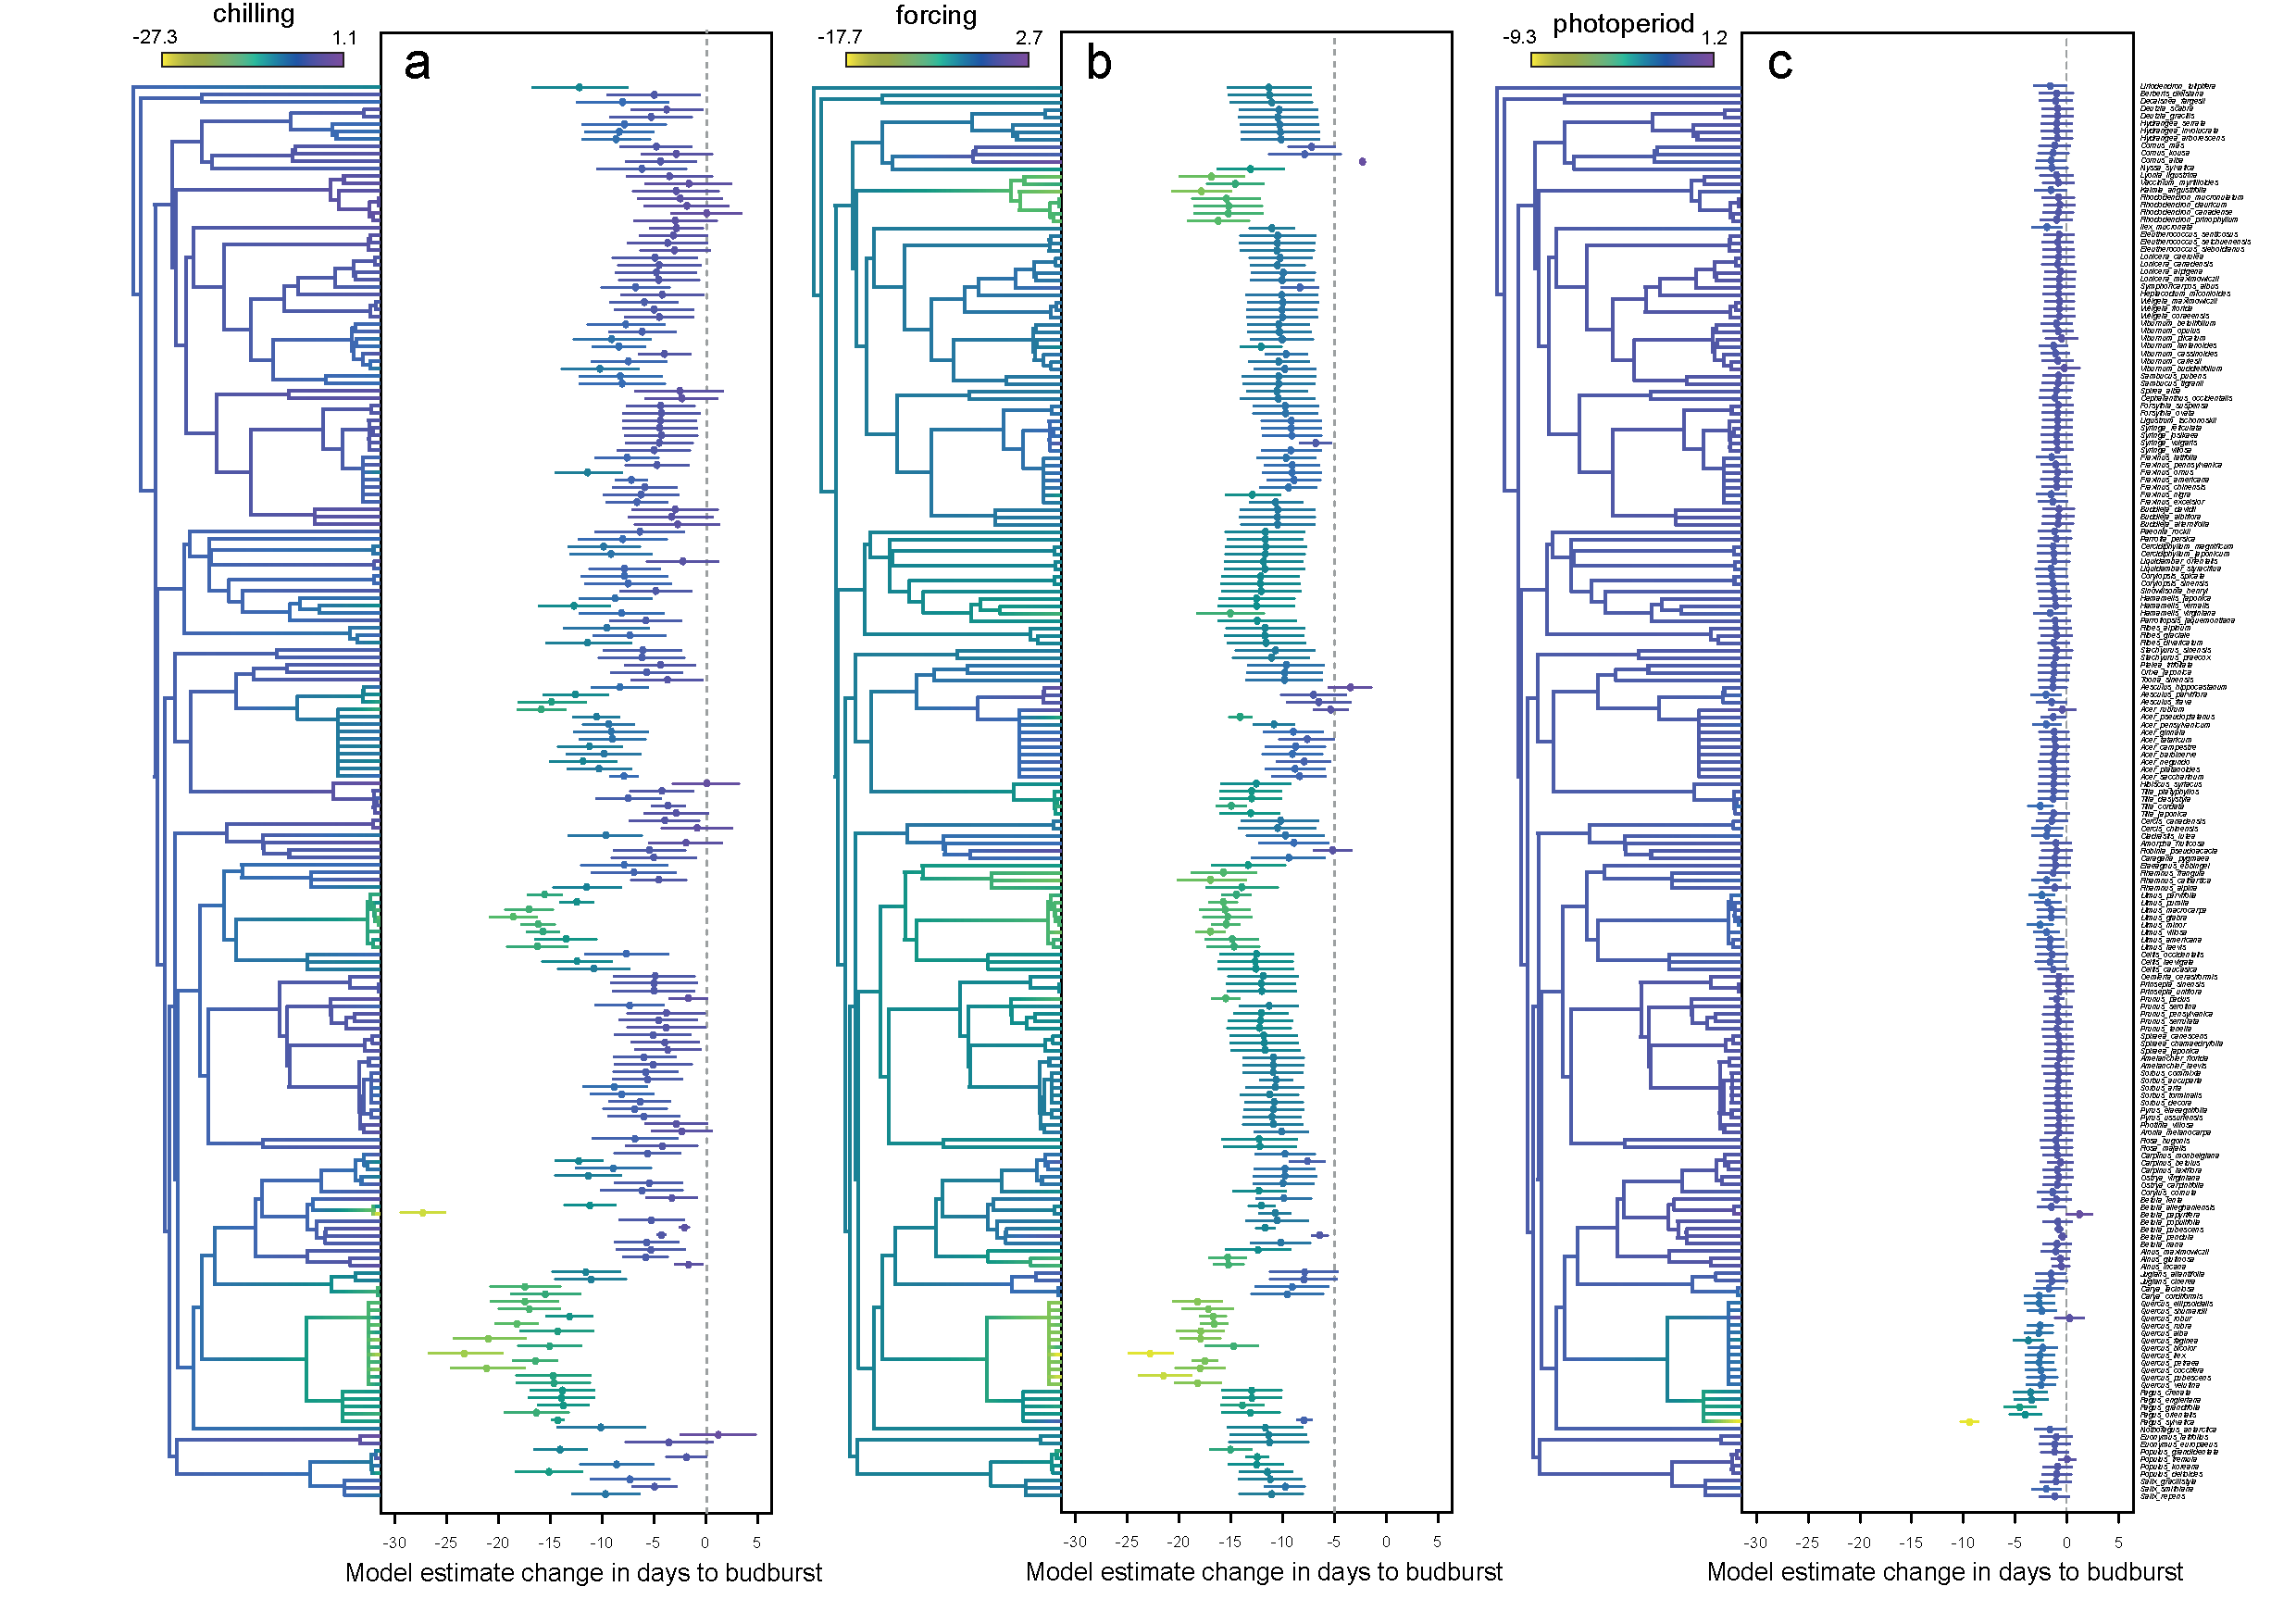
\includegraphics[width=16cm]{../../analyses/phylogeny/figures/Fig1_phylo_muplots191.pdf}
  \caption{Phenological sensitivity to three environmental cues, chilling (a), forcing (b) and photoperiod (c) measured in change in days to budburst per standardized unit (z-transformation) of the cues across 191 tree species. The same phylogenetic tree is shown in each panel, colored acording to an estimation of ancestral character states, being the states at the tips the species' sensitivities to a cue, as estimated by our hierarchical phylogenetic model. Species sensitivities are shown along with 50\% uncertainty intervals in the diagrams. Note that the color scale varies in each panel. Total tree depth is 81. My.}
  \label{fig:muplot_all}
  \end{center}
\end{figure}

\clearpage

\begin{figure} 
  \begin{center}
  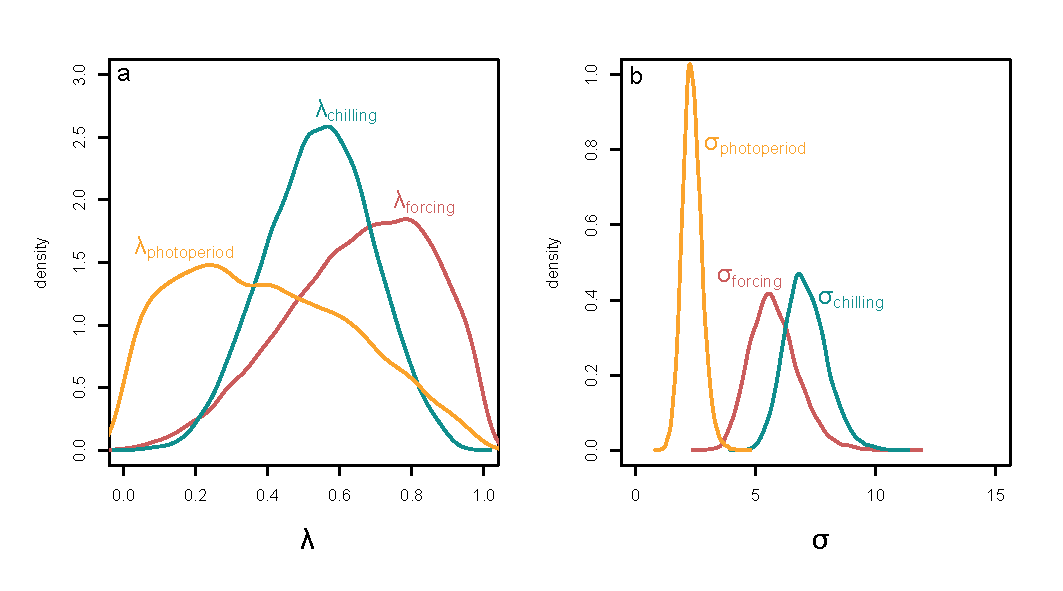
\includegraphics[width=14cm]{../../analyses/phylogeny/figures/Fig2_lambdas_sigmas.pdf}
  \caption{Density plots comparing the posterior distributions of phylogenetic parameters $\lambda$ and $\sigma$ estimated for each cue in the model: chilling (blue), forcing (red), and photoperiod (orange). Panels correspond to $\lambda$ (a) and $\sigma$ (b) from the phylogenetic model.}
  \label{fig:phylosig_all}
  \end{center}
\end{figure}

\begin{figure} 
  \begin{center}
  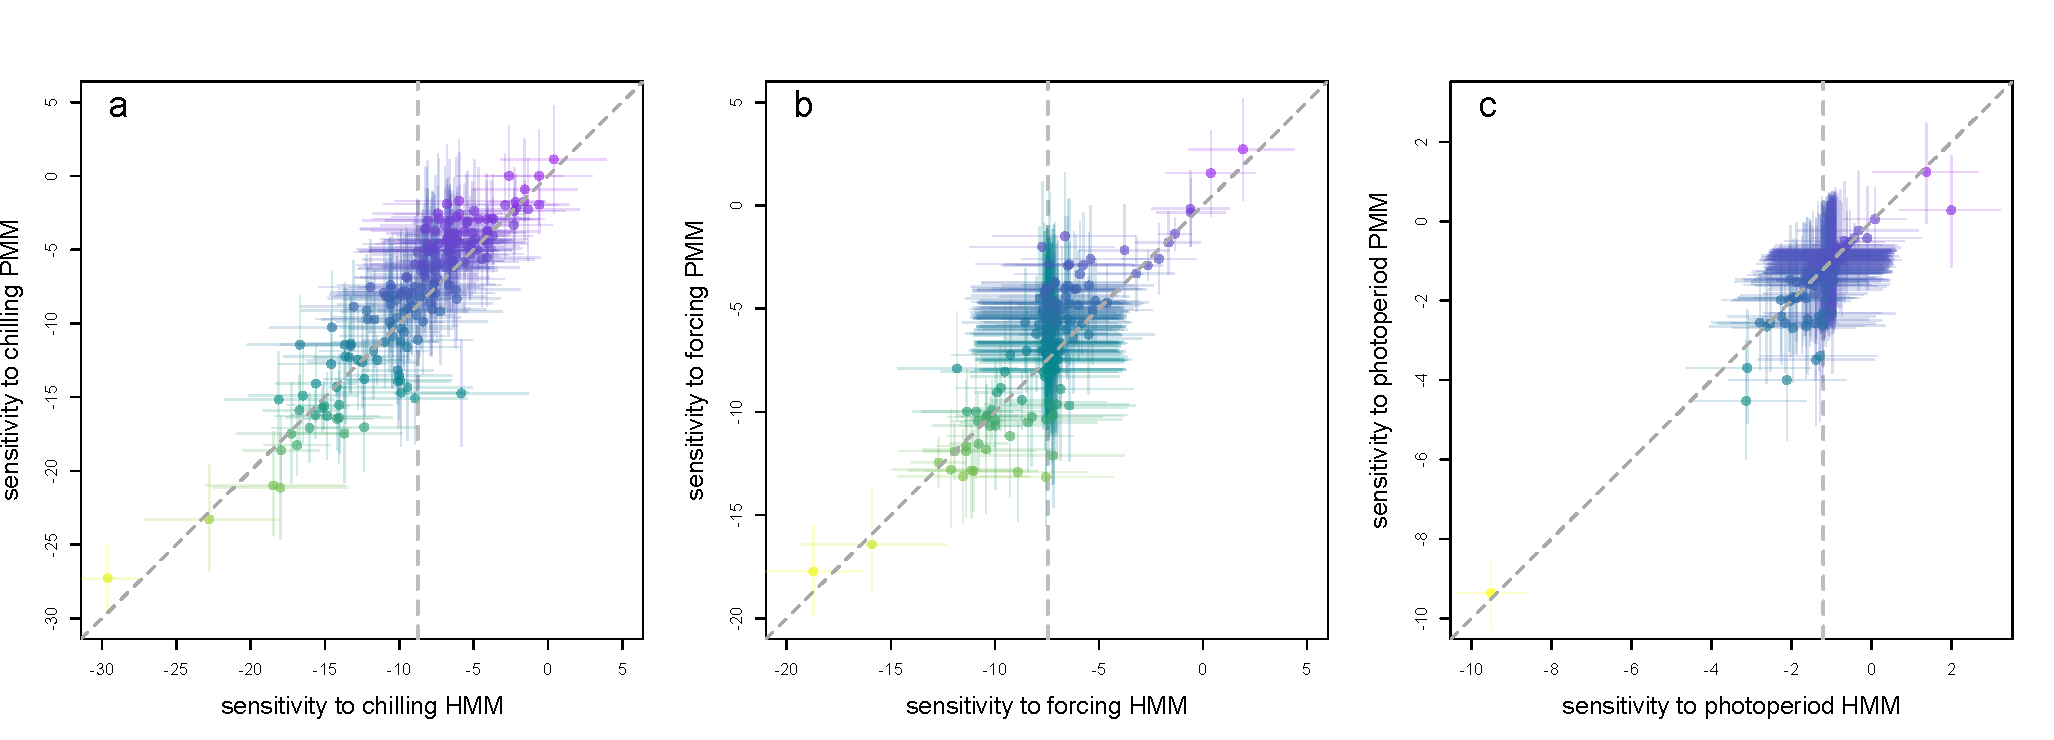
\includegraphics[width=14cm]{../../analyses/phylogeny/figures/Fig3_correlations_lambestvslamb0_cols.pdf}
  \caption{Correlations between model parameters as estimated by the model including phylogenetic structure on each phenological cue ($y$-axis), and the more commonly used hierarchical model where species are exchangeable (where $\lambda$ is constrained to be equal to zero, $x$-axis). While species with large amounts of data may be estimated similarly by both models, in the more commonly used hierarchical model ($x$-axis) many species are pulled towards the overall average (shown by dashed black horizontal lines). The strength and prevalence of pulling across species is particularly obvious for forcing (b). Panels correspond to sensitivity to chilling (a), forcing (b), and photoperiod (c). Dashed grey 1:1 lines also shown (with intercept equal zero and slope equal one).}
  \label{fig:correls_angio}
  \end{center}
\end{figure}




\begin{figure} 
  \begin{center}
  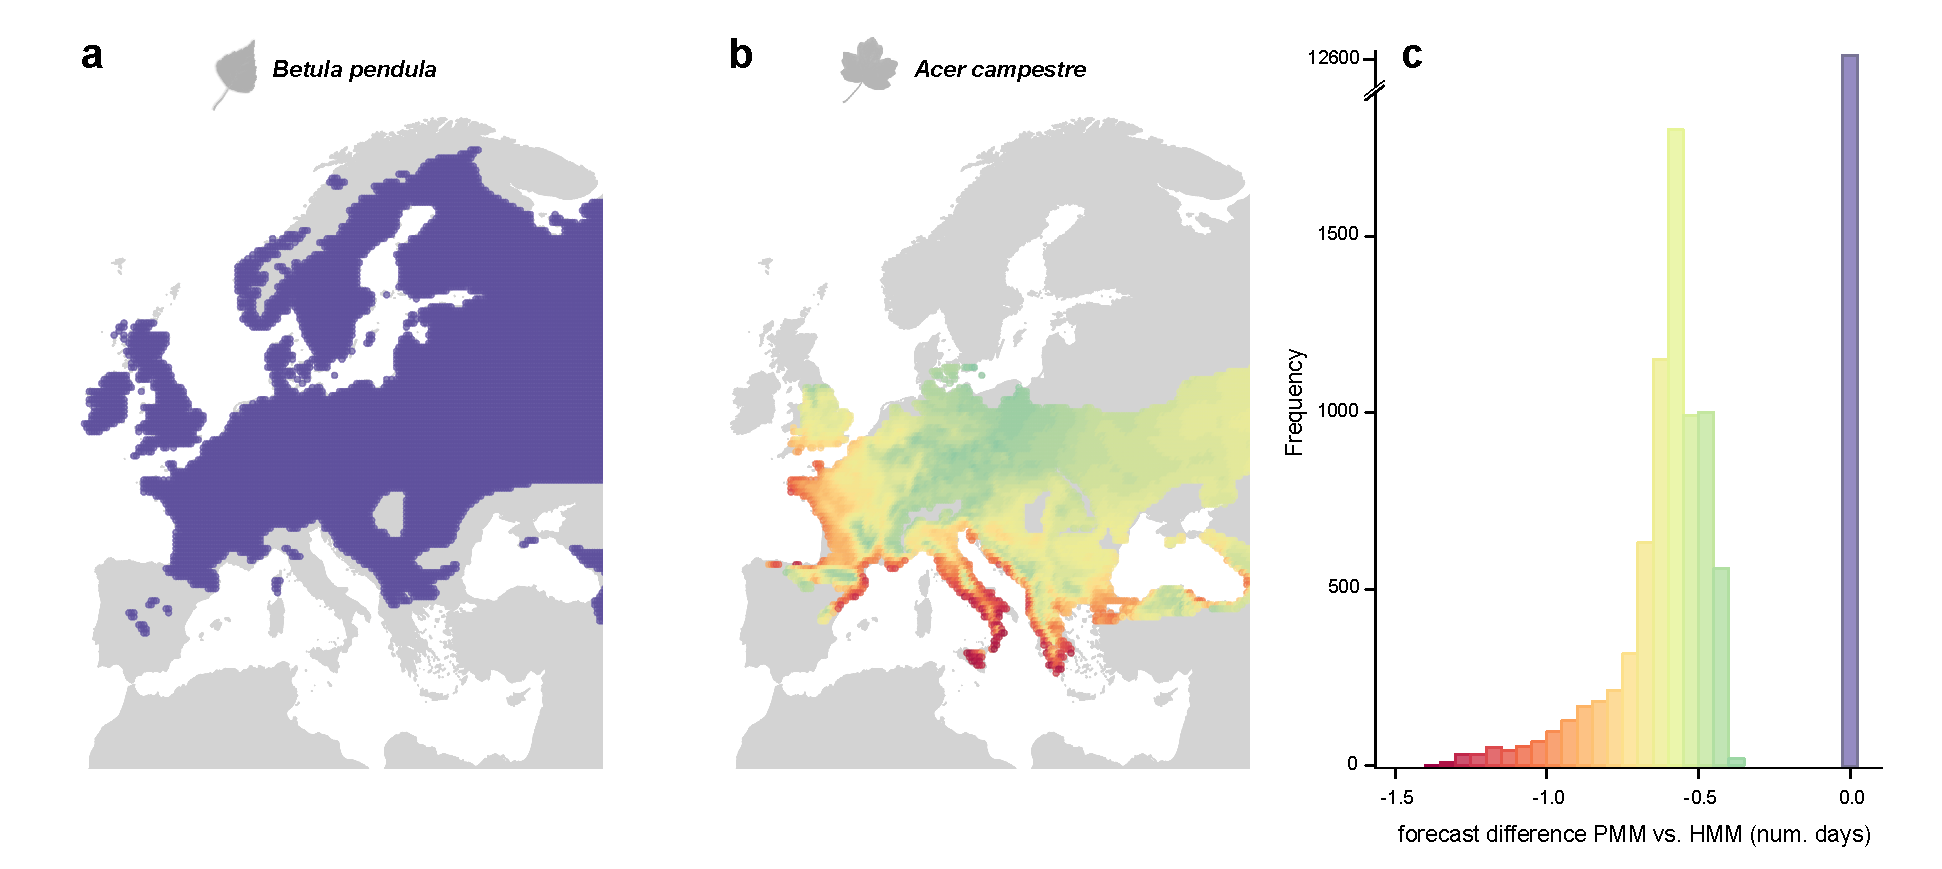
\includegraphics[width=16cm]{../../analyses/phylogeny/figures/Fig4_forecasting_diffstdpmm-lmm.pdf}
  \caption{Comparison of forecasts of phenological shifts (i.e., computed as the difference between predictions under current climate vs. a 2\$^{\circ}$C warmer climate) resulting from a phylogenetic (PMM) and a non-phylogenetic (HMM) approach. Forecasted shifts are negligible for well sampled species (\emph{Betula pendula}, n = 311, a), but can be substantially different for poorly sampled species in well-sampled clades (\emph{Acer campestre}, n = 6, b). The maps show the difference in number of days (relative to start of forcing conditions, not calendar days) between the shifts predicted by PMM and HMM, with values colored according to histograms in panel c. }
  \label{fig:forecast}
  \end{center}
\end{figure}

\clearpage




\end{document}
